\documentclass{beamer}\usepackage[]{graphicx}\usepackage[]{color}
%% maxwidth is the original width if it is less than linewidth
%% otherwise use linewidth (to make sure the graphics do not exceed the margin)
\makeatletter
\def\maxwidth{ %
  \ifdim\Gin@nat@width>\linewidth
    \linewidth
  \else
    \Gin@nat@width
  \fi
}
\makeatother

\definecolor{fgcolor}{rgb}{1, 0.894, 0.769}
\newcommand{\hlnum}[1]{\textcolor[rgb]{0.824,0.412,0.118}{#1}}%
\newcommand{\hlstr}[1]{\textcolor[rgb]{1,0.894,0.71}{#1}}%
\newcommand{\hlcom}[1]{\textcolor[rgb]{0.824,0.706,0.549}{#1}}%
\newcommand{\hlopt}[1]{\textcolor[rgb]{1,0.894,0.769}{#1}}%
\newcommand{\hlstd}[1]{\textcolor[rgb]{1,0.894,0.769}{#1}}%
\newcommand{\hlkwa}[1]{\textcolor[rgb]{0.941,0.902,0.549}{#1}}%
\newcommand{\hlkwb}[1]{\textcolor[rgb]{0.804,0.776,0.451}{#1}}%
\newcommand{\hlkwc}[1]{\textcolor[rgb]{0.78,0.941,0.545}{#1}}%
\newcommand{\hlkwd}[1]{\textcolor[rgb]{1,0.78,0.769}{#1}}%
\let\hlipl\hlkwb

\usepackage{framed}
\makeatletter
\newenvironment{kframe}{%
 \def\at@end@of@kframe{}%
 \ifinner\ifhmode%
  \def\at@end@of@kframe{\end{minipage}}%
  \begin{minipage}{\columnwidth}%
 \fi\fi%
 \def\FrameCommand##1{\hskip\@totalleftmargin \hskip-\fboxsep
 \colorbox{shadecolor}{##1}\hskip-\fboxsep
     % There is no \\@totalrightmargin, so:
     \hskip-\linewidth \hskip-\@totalleftmargin \hskip\columnwidth}%
 \MakeFramed {\advance\hsize-\width
   \@totalleftmargin\z@ \linewidth\hsize
   \@setminipage}}%
 {\par\unskip\endMakeFramed%
 \at@end@of@kframe}
\makeatother

\definecolor{shadecolor}{rgb}{.97, .97, .97}
\definecolor{messagecolor}{rgb}{0, 0, 0}
\definecolor{warningcolor}{rgb}{1, 0, 1}
\definecolor{errorcolor}{rgb}{1, 0, 0}
\newenvironment{knitrout}{}{} % an empty environment to be redefined in TeX

\usepackage{alltt}
\usepackage{../371g-slides}
\title{Multiple Regression}
\subtitle{Lecture 12}
\author{STA 371G}
\IfFileExists{upquote.sty}{\usepackage{upquote}}{}
\begin{document}
  
  
  

  \frame{\maketitle}

  % Show outline at beginning of each section
  \AtBeginSection[]{
    \begin{frame}<beamer>
      \tableofcontents[currentsection]
    \end{frame}
  }

  %%%%%%% Slides start here %%%%%%%

  \begin{darkframes}
    \begin{frame}
      How do you know how much a house is worth? \pause

      Zillow? How do they know?

      \begin{center}
        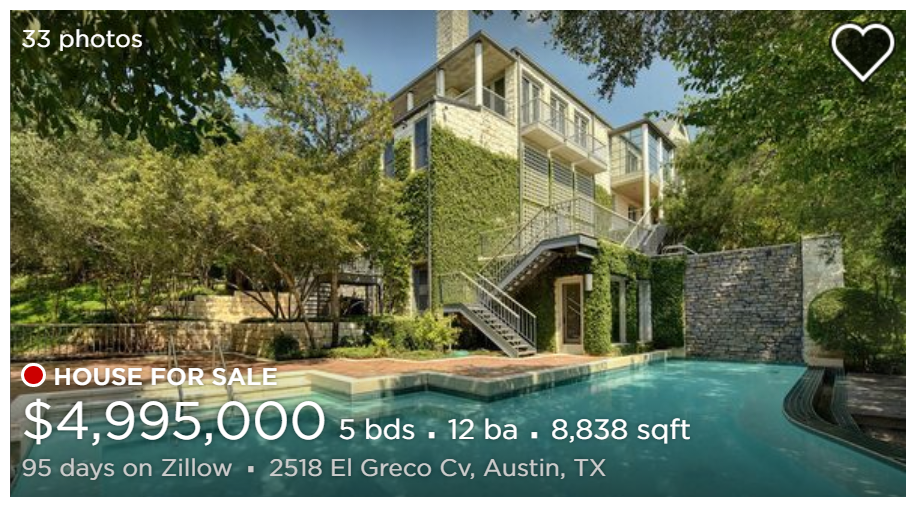
\includegraphics[width=3.5in]{zillow} \\
      \end{center} \pause

      \begin{columns}[onlytextwidth]
        \column{.5\textwidth}
          \begin{itemize}
            \item Square feet
            \item Year built
            \item \# of rooms
          \end{itemize}
        \column{.5\textwidth}
          \begin{itemize}
            \item Distance to downtown
            \item Crime rate
            \item ...
          \end{itemize}
      \end{columns}


    \end{frame}






    \begin{frame}

      \begin{center}
        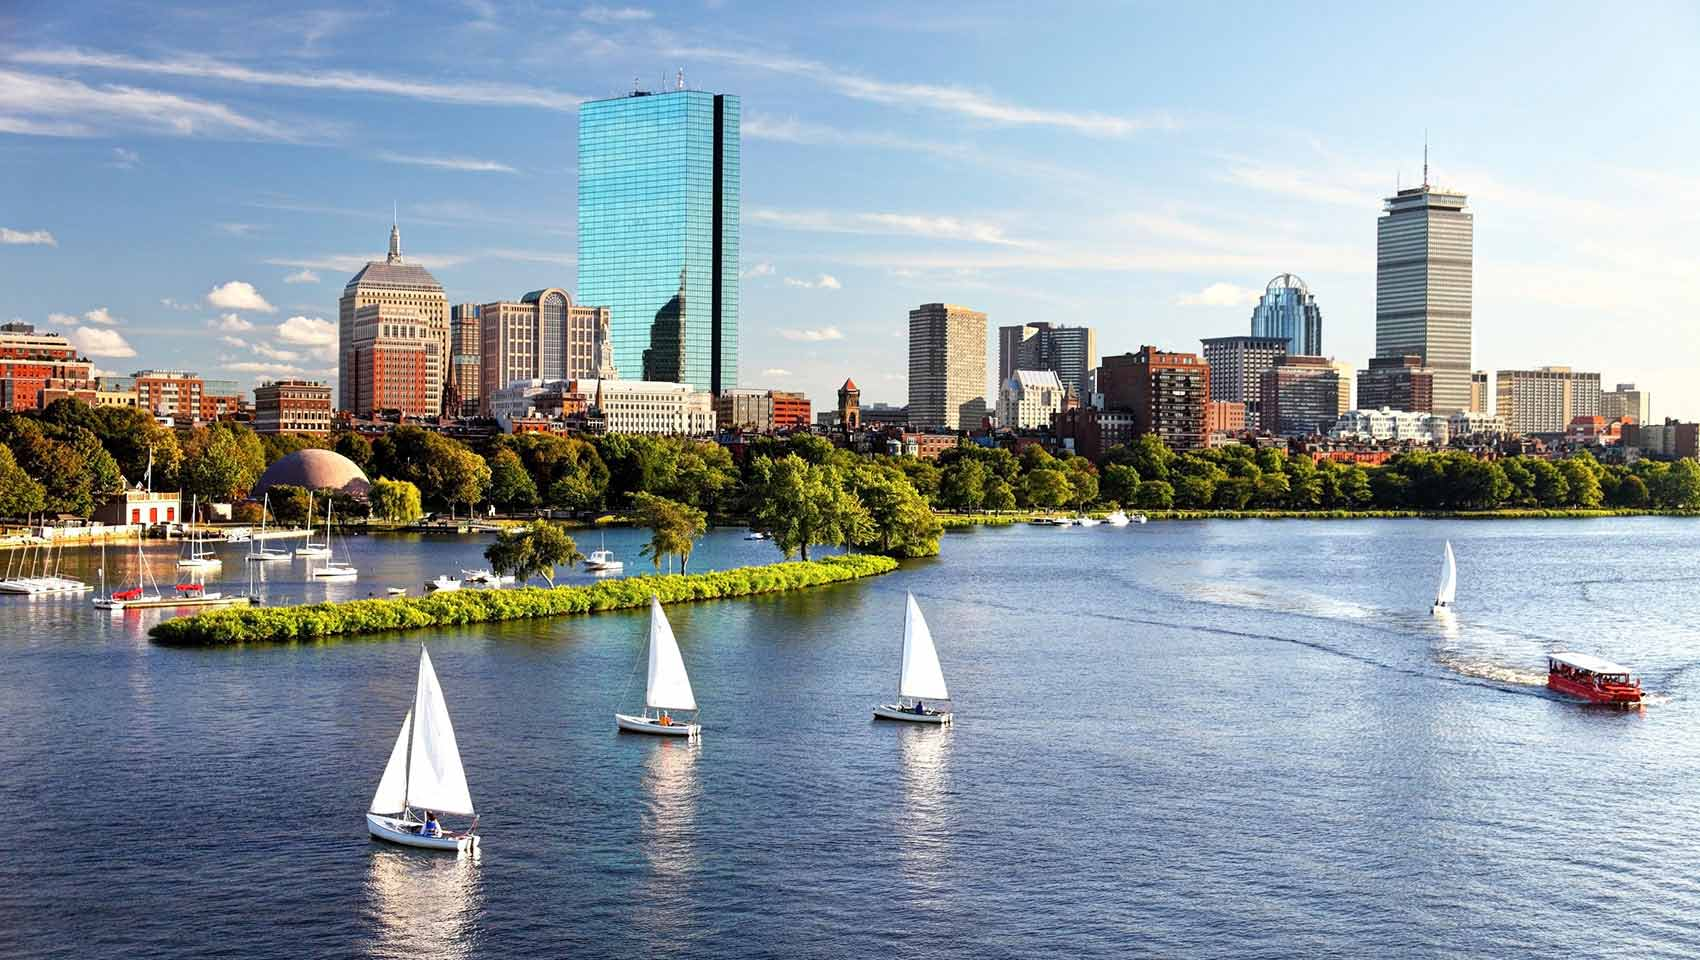
\includegraphics[width=4in]{boston} \\
      \end{center}

      Boston house price data (by census tract, 1970)
      \note{Every row corresponds to a census tract. The prices are multiplied by 20 to make them more relevant.}
    \end{frame}







    \begin{frame}

      \begin{columns}[onlytextwidth]
        \column{.5\textwidth}
          \begin{itemize}
            \item MEDV: Median Price (response)
            \item LON: Longitude
            \item LAT: Latitude
            \item CRIME: Per capita crime rate
            \item ZONE: Proportion of large lots
            \item INDUS: Proportion of non-retail business acres
            \item NOX: Nitrogen Oxide concentration
          \end{itemize}
        \column{.5\textwidth}
          \begin{itemize}
            \item ROOM: Average \# of rooms
            \item AGE: Proportion of built before 1940
            \item DIST: Distance to employment centers
            \item RADIAL: Accessibility to highways
            \item TAX: Tax rate (per \$10K)
            \item PTRATIO: Pupil-to-teacher ratio
            \item LSTAT: Proportion of ``lower status''
            %  proportion of adults without some high school education or that are classified as laborers
          \end{itemize}
      \end{columns}

    \end{frame}





    \begin{frame}
        Can you guess the top three factors?
        \lc
    \end{frame}




    \begin{frame}[fragile]{Distribution of house prices (MEDV)}
      \fontsize{10}{10}\selectfont
\begin{knitrout}
\definecolor{shadecolor}{rgb}{0.137, 0.137, 0.137}\begin{kframe}
\begin{alltt}
\hlstd{> }\hlkwd{hist}\hlstd{(boston}\hlopt{$}\hlstd{MEDV,} \hlkwc{col}\hlstd{=}\hlstr{'green'}\hlstd{,}
\hlstd{+ }  \hlkwc{main}\hlstd{=}\hlstr{''}\hlstd{,} \hlkwc{xlab}\hlstd{=}\hlstr{'Census Tract Median House Price'}\hlstd{)}
\end{alltt}
\end{kframe}
\input{/tmp/figures/unnamed-chunk-3-1.tikz}

\end{knitrout}
      \note{Not a normal distribution... We can mention log-normal distributions.}
    \end{frame}


        \begin{frame}{Multiple Regression Model}

      We model the median price in a census tract ($y_i=$ median price in $i$th tract) as a linear function of multiple predictors, plus some error.

      \[
        y_i = \beta_0 + \beta_1 x_{i1} + \beta_2 x_{i2} +\ldots + \beta_{13} x_{i13} + \epsilon_i
      \]

    \begin{table}[!b]
        {\carlitoTLF % Use monospaced lining figures
        \begin{tabularx}{\textwidth}{Xrrrrrr}

           & $\beta_0$ & $\beta_1$ & $\beta_2$ & \textbf{...} &   $\beta_{13}$ & \\
          \toprule

          & & \textbf{LAT} & \textbf{LON} & \textbf{...} &   \textbf{LSTAT} & \textbf{error}\\
          \toprule
    $y_1$ & 1 & $x_{1,1}$ & $x_{1,2}$  & \textbf{...} & $x_{1,13}$ & $\epsilon_1$  \\
    $y_2$ & 1 & $x_{2,1}$ & $x_{2,2}$  & \textbf{...} & $x_{2,13}$ & $\epsilon_2$\\
    \textbf{...}  & \textbf{...} &  \textbf{...} & \textbf{...}  & \textbf{...} &   \textbf{...}  & \textbf{...}\\
    %$y_{503}$ & 1 &  $x_{503,1}$ & $x_{503,2}$  & \textbf{...} &   $x_{503,13}$  & $\epsilon_{503}$\\

          \bottomrule
        \end{tabularx}}

      \end{table}

      \bigskip\pause

      We find $\hat\beta_0,\ldots,\hat\beta_{13}$ to minimize the residuals ($y_i-\hat y_i$)

      %\[
      %  \hat y_i = \hat\beta_0 + \hat\beta_1 x_{i1} + \hat\beta_2 x_{i2} +\ldots + \hat\beta_{13} x_{i13}
      %\]
    \end{frame}





    \begin{frame}[fragile]
      \fontsize{9}{9}\selectfont
\begin{knitrout}
\definecolor{shadecolor}{rgb}{0.137, 0.137, 0.137}\begin{kframe}
\begin{alltt}
\hlstd{> }\hlstd{model} \hlkwb{<-} \hlkwd{lm}\hlstd{(MEDV} \hlopt{~} \hlstd{LON}\hlopt{+}\hlstd{LAT}\hlopt{+}\hlstd{CRIME}\hlopt{+}\hlstd{ZONE}\hlopt{+}\hlstd{INDUS}\hlopt{+}\hlstd{NOX}\hlopt{+}\hlstd{ROOM}\hlopt{+}\hlstd{AGE}\hlopt{+}\hlstd{DIST}
\hlstd{+ }                  \hlopt{+}\hlstd{RADIAL}\hlopt{+}\hlstd{TAX}\hlopt{+}\hlstd{PTRATIO}\hlopt{+}\hlstd{LSTAT,} \hlkwc{data}\hlstd{=boston)}
\hlstd{> }\hlkwd{summary}\hlstd{(model}\hlopt{$}\hlstd{residuals)}
\end{alltt}
\begin{verbatim}
   Min. 1st Qu.  Median    Mean 3rd Qu.    Max. 
-258106  -57337  -13642       0   39614  531268 
\end{verbatim}
\begin{alltt}
\hlstd{> }\hlkwd{summary}\hlstd{(model)}\hlopt{$}\hlstd{r.squared}
\end{alltt}
\begin{verbatim}
[1] 0.7305487
\end{verbatim}
\begin{alltt}
\hlstd{> }\hlkwd{summary}\hlstd{(model)}\hlopt{$}\hlstd{adj.r.squared}
\end{alltt}
\begin{verbatim}
[1] 0.7234291
\end{verbatim}
\end{kframe}
\end{knitrout}
      This is a high $R^2$ compared to the prior examples!

      Keep an eye on the Adjusted-$R^2$...
    \end{frame}


    \begin{frame}[fragile]
      Here is how the predictors contribute to the estimation:
      \fontsize{9}{9}\selectfont
\begin{knitrout}
\definecolor{shadecolor}{rgb}{0.137, 0.137, 0.137}\begin{kframe}
\begin{alltt}
\hlstd{> }\hlkwd{round}\hlstd{(}\hlkwd{summary}\hlstd{(model)}\hlopt{$}\hlstd{coefficients,}\hlnum{3}\hlstd{)}
\end{alltt}
\begin{verbatim}
                 Estimate  Std. Error t value Pr(>|t|)
(Intercept) -10815106.841 6202196.194  -1.744    0.082
LON           -100538.327   68540.103  -1.467    0.143
LAT            105813.832   75439.531   1.403    0.161
CRIME           -2497.915     665.762  -3.752    0.000
ZONE              920.725     282.649   3.257    0.001
INDUS             447.859    1267.151   0.353    0.724
NOX           -320021.023   82010.164  -3.902    0.000
ROOM            72906.394    8529.875   8.547    0.000
AGE               167.225     273.353   0.612    0.541
DIST           -27489.610    4295.791  -6.399    0.000
RADIAL           6274.465    1362.945   4.604    0.000
TAX              -286.853      76.087  -3.770    0.000
PTRATIO        -18304.240    2801.930  -6.533    0.000
LSTAT          -11416.450    1022.127 -11.169    0.000
\end{verbatim}
\end{kframe}
\end{knitrout}
      \quad \pause

      Intercept, INDUS, AGE, LAT and LON seem to be statistically insignificant. Should we omit them altogether?
    \end{frame}


    \begin{frame}
      
      Let's interpret the ROOM coefficient 72906.39. The interpretation is:
      \begin{itemize}[<+->]
        \item \emph{Holding the other predictors (X variables) constant}, our predicted home price increases by \$72906.39 for each additional room.
        \item Two census tracts that are otherwise identical (but where one census tract has 1 more room on average than the other) will differ by \$72906.39 in their predicted home price.
      \end{itemize}
    \end{frame}



    \begin{frame}
      A $p$-value of predictor $i$ tests the null hypothesis that $\beta_i=0$; i.e., that predictor $i$ has no contribution to predicting $Y$ independent above and beyond the other predictors

      \bigskip

      Omitting other predictors might increase the significance (decrease the $p$-value) of a statistically insignificant predictor.
    \end{frame}


    \begin{frame}[fragile]
      \fontsize{9}{9}\selectfont
\begin{knitrout}
\definecolor{shadecolor}{rgb}{0.137, 0.137, 0.137}\begin{kframe}
\begin{alltt}
\hlstd{> }\hlstd{model_red} \hlkwb{<-} \hlkwd{lm}\hlstd{(MEDV} \hlopt{~} \hlstd{LON}\hlopt{+}\hlstd{LAT}\hlopt{+}\hlstd{INDUS}\hlopt{+}\hlstd{AGE,} \hlkwc{data}\hlstd{=boston)}
\hlstd{> }\hlkwd{round}\hlstd{(}\hlkwd{summary}\hlstd{(model_red)}\hlopt{$}\hlstd{coefficients,}\hlnum{3}\hlstd{)}
\end{alltt}
\begin{verbatim}
                 Estimate  Std. Error t value Pr(>|t|)
(Intercept) -54327833.818 8559058.342  -6.347    0.000
LON           -709317.003   92858.638  -7.639    0.000
LAT            107180.101  111629.613   0.960    0.337
INDUS          -11817.533    1305.467  -9.052    0.000
AGE              -235.769     324.422  -0.727    0.468
\end{verbatim}
\begin{alltt}
\hlstd{> }\hlkwd{summary}\hlstd{(model_red)}\hlopt{$}\hlstd{r.squared}
\end{alltt}
\begin{verbatim}
[1] 0.3203884
\end{verbatim}
\end{kframe}
\end{knitrout}
      LON and INDUS look like a big deal now, although they do not explain as much with $R^2=0.32$.

      Let's start omiting one by one.
    \end{frame}




    \begin{frame}[fragile]
      \fontsize{9}{9}\selectfont
      INDUS has been omitted.
\begin{knitrout}
\definecolor{shadecolor}{rgb}{0.137, 0.137, 0.137}\begin{kframe}
\begin{alltt}
\hlstd{> }\hlstd{model} \hlkwb{<-} \hlkwd{lm}\hlstd{(MEDV} \hlopt{~} \hlstd{LON}\hlopt{+}\hlstd{LAT}\hlopt{+}\hlstd{CRIME}\hlopt{+}\hlstd{ZONE}\hlopt{+}\hlstd{NOX}\hlopt{+}\hlstd{ROOM}\hlopt{+}\hlstd{AGE}\hlopt{+}\hlstd{DIST}
\hlstd{+ }                  \hlopt{+}\hlstd{RADIAL}\hlopt{+}\hlstd{TAX}\hlopt{+}\hlstd{PTRATIO}\hlopt{+}\hlstd{LSTAT,} \hlkwc{data}\hlstd{=boston)}
\hlstd{> }\hlkwd{summary}\hlstd{(model)}\hlopt{$}\hlstd{r.squared}
\end{alltt}
\begin{verbatim}
[1] 0.7304803
\end{verbatim}
\begin{alltt}
\hlstd{> }\hlkwd{summary}\hlstd{(model)}\hlopt{$}\hlstd{adj.r.squared}
\end{alltt}
\begin{verbatim}
[1] 0.72392
\end{verbatim}
\end{kframe}
\end{knitrout}
      $R^2$ has not changed too much, Adjusted-$R^2$ has increased a bit.
    \end{frame}


    \begin{frame}[fragile]
      \fontsize{9}{9}\selectfont
\begin{knitrout}
\definecolor{shadecolor}{rgb}{0.137, 0.137, 0.137}\begin{kframe}
\begin{alltt}
\hlstd{> }\hlkwd{round}\hlstd{(}\hlkwd{summary}\hlstd{(model)}\hlopt{$}\hlstd{coefficients,}\hlnum{3}\hlstd{)}
\end{alltt}
\begin{verbatim}
                 Estimate  Std. Error t value Pr(>|t|)
(Intercept) -11078358.838 6151842.621  -1.801    0.072
LON           -104687.251   67467.423  -1.552    0.121
LAT            104977.262   75335.440   1.393    0.164
CRIME           -2504.206     664.933  -3.766    0.000
ZONE              907.905     280.062   3.242    0.001
NOX           -311362.657   78196.317  -3.982    0.000
ROOM            72586.523    8474.196   8.566    0.000
AGE               170.953     272.907   0.626    0.531
DIST           -27725.142    4240.019  -6.539    0.000
RADIAL           6136.632    1304.802   4.703    0.000
TAX              -275.379      68.753  -4.005    0.000
PTRATIO        -18137.431    2759.443  -6.573    0.000
LSTAT          -11391.407    1018.762 -11.182    0.000
\end{verbatim}
\end{kframe}
\end{knitrout}


      AGE still seems insignificant.
    \end{frame}





    \begin{frame}[fragile]
      \fontsize{9}{9}\selectfont
      AGE has been omitted.
\begin{knitrout}
\definecolor{shadecolor}{rgb}{0.137, 0.137, 0.137}\begin{kframe}
\begin{alltt}
\hlstd{> }\hlstd{model} \hlkwb{<-} \hlkwd{lm}\hlstd{(MEDV} \hlopt{~} \hlstd{LON}\hlopt{+}\hlstd{LAT}\hlopt{+}\hlstd{CRIME}\hlopt{+}\hlstd{ZONE}\hlopt{+}\hlstd{NOX}\hlopt{+}\hlstd{ROOM}\hlopt{+}\hlstd{DIST}
\hlstd{+ }                  \hlopt{+}\hlstd{RADIAL}\hlopt{+}\hlstd{TAX}\hlopt{+}\hlstd{PTRATIO}\hlopt{+}\hlstd{LSTAT,} \hlkwc{data}\hlstd{=boston)}
\hlstd{> }\hlkwd{summary}\hlstd{(model)}\hlopt{$}\hlstd{r.squared}
\end{alltt}
\begin{verbatim}
[1] 0.7302658
\end{verbatim}
\begin{alltt}
\hlstd{> }\hlkwd{summary}\hlstd{(model)}\hlopt{$}\hlstd{adj.r.squared}
\end{alltt}
\begin{verbatim}
[1] 0.7242596
\end{verbatim}
\end{kframe}
\end{knitrout}
      $R^2$ is again about the same, and Adjusted-$R^2$ has increased a bit.
    \end{frame}


    \begin{frame}[fragile]
      \fontsize{9}{9}\selectfont
\begin{knitrout}
\definecolor{shadecolor}{rgb}{0.137, 0.137, 0.137}\begin{kframe}
\begin{alltt}
\hlstd{> }\hlkwd{round}\hlstd{(}\hlkwd{summary}\hlstd{(model)}\hlopt{$}\hlstd{coefficients,}\hlnum{3}\hlstd{)}
\end{alltt}
\begin{verbatim}
                 Estimate  Std. Error t value Pr(>|t|)
(Intercept) -10647181.257 6109452.440  -1.743    0.082
LON            -97363.810   66405.890  -1.466    0.143
LAT            107052.256   75216.281   1.423    0.155
CRIME           -2512.856     664.380  -3.782    0.000
ZONE              891.239     278.624   3.199    0.001
NOX           -300532.234   76214.057  -3.943    0.000
ROOM            73744.325    8265.087   8.922    0.000
DIST           -28594.368    4004.063  -7.141    0.000
RADIAL           6088.931    1301.777   4.677    0.000
TAX              -273.672      68.657  -3.986    0.000
PTRATIO        -18104.114    2757.233  -6.566    0.000
LSTAT          -11177.763     959.387 -11.651    0.000
\end{verbatim}
\end{kframe}
\end{knitrout}
      LAT is next.
    \end{frame}



    \begin{frame}[fragile]
      \fontsize{9}{9}\selectfont
      LAT has been omitted.
\begin{knitrout}
\definecolor{shadecolor}{rgb}{0.137, 0.137, 0.137}\begin{kframe}
\begin{alltt}
\hlstd{> }\hlstd{model} \hlkwb{<-} \hlkwd{lm}\hlstd{(MEDV} \hlopt{~} \hlstd{LON}\hlopt{+}\hlstd{CRIME}\hlopt{+}\hlstd{ZONE}\hlopt{+}\hlstd{NOX}\hlopt{+}\hlstd{ROOM}\hlopt{+}\hlstd{DIST}
\hlstd{+ }                  \hlopt{+}\hlstd{RADIAL}\hlopt{+}\hlstd{TAX}\hlopt{+}\hlstd{PTRATIO}\hlopt{+}\hlstd{LSTAT,} \hlkwc{data}\hlstd{=boston)}
\hlstd{> }\hlkwd{summary}\hlstd{(model)}\hlopt{$}\hlstd{r.squared}
\end{alltt}
\begin{verbatim}
[1] 0.7291597
\end{verbatim}
\begin{alltt}
\hlstd{> }\hlkwd{summary}\hlstd{(model)}\hlopt{$}\hlstd{adj.r.squared}
\end{alltt}
\begin{verbatim}
[1] 0.7236882
\end{verbatim}
\end{kframe}
\end{knitrout}
      Both $R^2$ and Adjusted-$R^2$ have reduced. But still not too bad.
    \end{frame}


    \begin{frame}[fragile]
      \fontsize{9}{9}\selectfont
\begin{knitrout}
\definecolor{shadecolor}{rgb}{0.137, 0.137, 0.137}\begin{kframe}
\begin{alltt}
\hlstd{> }\hlkwd{round}\hlstd{(}\hlkwd{summary}\hlstd{(model)}\hlopt{$}\hlstd{coefficients,}\hlnum{3}\hlstd{)}
\end{alltt}
\begin{verbatim}
                Estimate  Std. Error t value Pr(>|t|)
(Intercept) -5072210.579 4693368.926  -1.081    0.280
LON           -82749.985   65675.201  -1.260    0.208
CRIME          -2507.401     665.057  -3.770    0.000
ZONE             874.164     278.654   3.137    0.002
NOX          -318434.670   75246.742  -4.232    0.000
ROOM           73594.882    8272.978   8.896    0.000
DIST          -29692.314    3933.116  -7.549    0.000
RADIAL          5853.970    1292.603   4.529    0.000
TAX             -271.753      68.714  -3.955    0.000
PTRATIO       -18211.873    2759.048  -6.601    0.000
LSTAT         -11062.388     956.946 -11.560    0.000
\end{verbatim}
\end{kframe}
\end{knitrout}
      Bye LON...
    \end{frame}


    \begin{frame}[fragile]
      \fontsize{9}{9}\selectfont
      LON has been omitted.
\begin{knitrout}
\definecolor{shadecolor}{rgb}{0.137, 0.137, 0.137}\begin{kframe}
\begin{alltt}
\hlstd{> }\hlstd{model} \hlkwb{<-} \hlkwd{lm}\hlstd{(MEDV} \hlopt{~} \hlstd{CRIME}\hlopt{+}\hlstd{ZONE}\hlopt{+}\hlstd{NOX}\hlopt{+}\hlstd{ROOM}\hlopt{+}\hlstd{DIST}
\hlstd{+ }                  \hlopt{+}\hlstd{RADIAL}\hlopt{+}\hlstd{TAX}\hlopt{+}\hlstd{PTRATIO}\hlopt{+}\hlstd{LSTAT,} \hlkwc{data}\hlstd{=boston)}
\hlstd{> }\hlkwd{summary}\hlstd{(model)}\hlopt{$}\hlstd{r.squared}
\end{alltt}
\begin{verbatim}
[1] 0.7282911
\end{verbatim}
\begin{alltt}
\hlstd{> }\hlkwd{summary}\hlstd{(model)}\hlopt{$}\hlstd{adj.r.squared}
\end{alltt}
\begin{verbatim}
[1] 0.7233609
\end{verbatim}
\end{kframe}
\end{knitrout}
      Both $R^2$ and Adjusted-$R^2$ have reduced. But that's OK.
    \end{frame}


    \begin{frame}[fragile]
      \fontsize{9}{9}\selectfont
\begin{knitrout}
\definecolor{shadecolor}{rgb}{0.137, 0.137, 0.137}\begin{kframe}
\begin{alltt}
\hlstd{> }\hlkwd{round}\hlstd{(}\hlkwd{summary}\hlstd{(model)}\hlopt{$}\hlstd{coefficients,}\hlnum{3}\hlstd{)}
\end{alltt}
\begin{verbatim}
               Estimate Std. Error t value Pr(>|t|)
(Intercept)  840065.150  99001.032   8.485    0.000
CRIME         -2566.084    663.817  -3.866    0.000
ZONE            921.998    276.220   3.338    0.001
NOX         -346925.672  71811.323  -4.831    0.000
ROOM          74242.520   8261.884   8.986    0.000
DIST         -31049.529   3784.980  -8.203    0.000
RADIAL         6000.243   1288.142   4.658    0.000
TAX            -265.331     68.566  -3.870    0.000
PTRATIO      -19279.752   2627.204  -7.339    0.000
LSTAT        -11071.731    957.483 -11.563    0.000
\end{verbatim}
\end{kframe}
\end{knitrout}
      Notice what happened to the intercept. LON (and perhaps the others) was acting like an intercept!
    \end{frame}


    \begin{frame}{When to omit, when to keep?}
      It is usually good to omit statistically insignificant variables, because:
      \begin{itemize}
        \item The model gets simpler
        \item Insignificant variables may lead to incorrect interpretations (as in LON)
        \item When the data set is small, we can read too much into the impact of insignificant variables
      \end{itemize}

    \end{frame}

    \begin{frame}{When to omit, when to keep?}
      We keep a variable in the model, even if it is statistically insignificant, when:
      \begin{itemize}
        \item We are testing a hypothesis on the variable
        \item The variable has a big effect, although it is statistically insignificant
        \item It is an expected control variable (e.g. age in medical studies, race in sociological studies etc.)
        \item It is included in a higher order term (more on this later)

      \end{itemize}

    \end{frame}


    \begin{frame}{``Most important'' predictors}
      How to identify which predictors have ``more significant'' effect on the response?

      \begin{itemize}
        \item[] Parameter estimate? \pause
        \item[] $p$-value? \pause
        \item[] t score? \pause \greencheckmark

      \end{itemize}

    \end{frame}


    \begin{frame}[fragile]
      \fontsize{9}{9}\selectfont
      Which ones seem to be the most important?
\begin{knitrout}
\definecolor{shadecolor}{rgb}{0.137, 0.137, 0.137}\begin{kframe}
\begin{alltt}
\hlstd{> }\hlkwd{round}\hlstd{(}\hlkwd{summary}\hlstd{(model)}\hlopt{$}\hlstd{coefficients,}\hlnum{3}\hlstd{)}
\end{alltt}
\begin{verbatim}
               Estimate Std. Error t value Pr(>|t|)
(Intercept)  840065.150  99001.032   8.485    0.000
CRIME         -2566.084    663.817  -3.866    0.000
ZONE            921.998    276.220   3.338    0.001
NOX         -346925.672  71811.323  -4.831    0.000
ROOM          74242.520   8261.884   8.986    0.000
DIST         -31049.529   3784.980  -8.203    0.000
RADIAL         6000.243   1288.142   4.658    0.000
TAX            -265.331     68.566  -3.870    0.000
PTRATIO      -19279.752   2627.204  -7.339    0.000
LSTAT        -11071.731    957.483 -11.563    0.000
\end{verbatim}
\end{kframe}
\end{knitrout}
      \lc
    \end{frame}



  \end{darkframes}

\end{document}
